\documentclass[12pt]{article}
\usepackage[a4paper, bindingoffset=0.2in, %
left=0.5in,right=0.5in,top=0.5in,bottom=0.5in,%
footskip=.25in]{geometry}
\usepackage{graphicx}
\usepackage{listings}
\usepackage{amssymb}
\usepackage{hyperref}
\usepackage{subcaption}

\title{HW1 Report}
\author{Mohammad Jamshidi}
\date{}
\begin{document}
	\maketitle
	\section{Problem 1 [code is available at ]}
	In this problem I wrote a python code to make Koch snowflake fractal. Here I assume that the length of initial segment is equal to 1; but a completely similar apraoch can be used for an arbitrary initial length, a. For building this fractal I used following rules:
	\begin{enumerate}
		\item 
		Scale all lengths with scaling factor $\frac{1}{3}$.
		\item 
		Rotate all segments in the anticlockwise direction for 60 degrees. Then Scale all lengths with scaling factor $\frac{1}{3}$. Finaly transfer the shape to the +x direction for $\frac{1}{3}$.
		\item 
		Rotate all segments in the clockwise direction for 60 degrees. Then Scale all lengths with scaling factor $\frac{1}{3}$. After all, transfer the shape to the +x direction for $\frac{1}{2}$ and then transfer it to the +y direction for $\frac{\sqrt{3}}{6}$.
		\item 
		Finally Scale all lengths with scaling factor $\frac{1}{3}$ and transfer them for $\frac{2}{3}$ to the +x direction.
	\end{enumerate}
	\begin{figure}[ht]
	\begin{subfigure}{0.5\textwidth}
	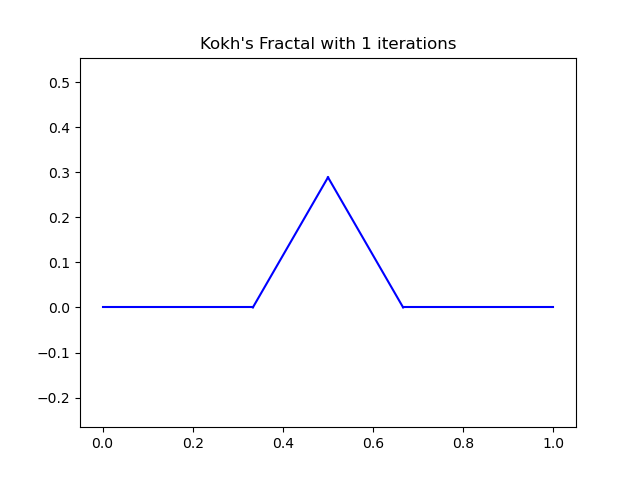
\includegraphics[width=0.8\linewidth]{1.1.png}
	\end{subfigure}
	\end{figure}
\end{document}
